\documentclass{article}
\usepackage[margin=1in]{geometry}
\usepackage{amsmath}
\usepackage{amssymb}
\usepackage{amsthm}
\usepackage{bm}
\usepackage{hyperref}
\usepackage{graphicx}
\usepackage{caption}
\usepackage{listings}
\usepackage{xcolor}
\usepackage{float}
\usepackage{placeins}
\graphicspath{{figures/}}

% Code style
\lstdefinestyle{code}{
  basicstyle=\ttfamily\small,
  numbers=left,
  numberstyle=\tiny,
  numbersep=8pt,
  keywordstyle=\color{blue},
  commentstyle=\color{teal!70!black},
  stringstyle=\color{orange!70!black},
  showstringspaces=false,
  breaklines=true,
  frame=single,
  framerule=0.3pt,
  rulecolor=\color{black!15}
}
\lstset{style=code}

\title{Foundations of Neural Networks}
\author{}
\date{\today}

\begin{document}
\maketitle
\tableofcontents
\FloatBarrier

\section{Artificial Neuron Model (Perceptron)}
The perceptron is the simplest artificial neuron. It computes a linear combination of inputs and passes the result through a step function to obtain a binary output. Formally, for input vector $\mathbf{x}=[x_1,\ldots,x_d]^\top$, weight vector $\mathbf{w}=[w_1,\ldots,w_d]^\top$, and bias $b$, the perceptron output is
\begin{equation}
  y = \mathrm{sign}\left(\mathbf{w}^\top \mathbf{x} + b\right),
\end{equation}
where $\mathrm{sign}(z) = 1$ if $z\geq0$ and $-1$ otherwise. The hyperplane $\mathbf{w}^\top\mathbf{x}+b=0$ partitions the input space into two classes.

\subsection{Learning Rule}
The classic perceptron learning algorithm performs stochastic gradient descent on the hinge-like loss by updating weights when a mistake occurs on a labeled example $(\mathbf{x}, t)$ with $t\in\{-1,1\}$. The update reads
\begin{equation}
  \mathbf{w} \leftarrow \mathbf{w} + \eta t \mathbf{x}, \quad b \leftarrow b + \eta t,
\end{equation}
with learning rate $\eta>0$. The update encourages the decision boundary to move toward correctly classifying the mispredicted point. Convergence is guaranteed if the data are linearly separable.

\subsection{Geometric Intuition}
Figure~\ref{fig:perceptron_decision_boundary} illustrates the perceptron decision boundary and the signed distances of points from the separating hyperplane.

\begin{figure}[H]
  \centering
  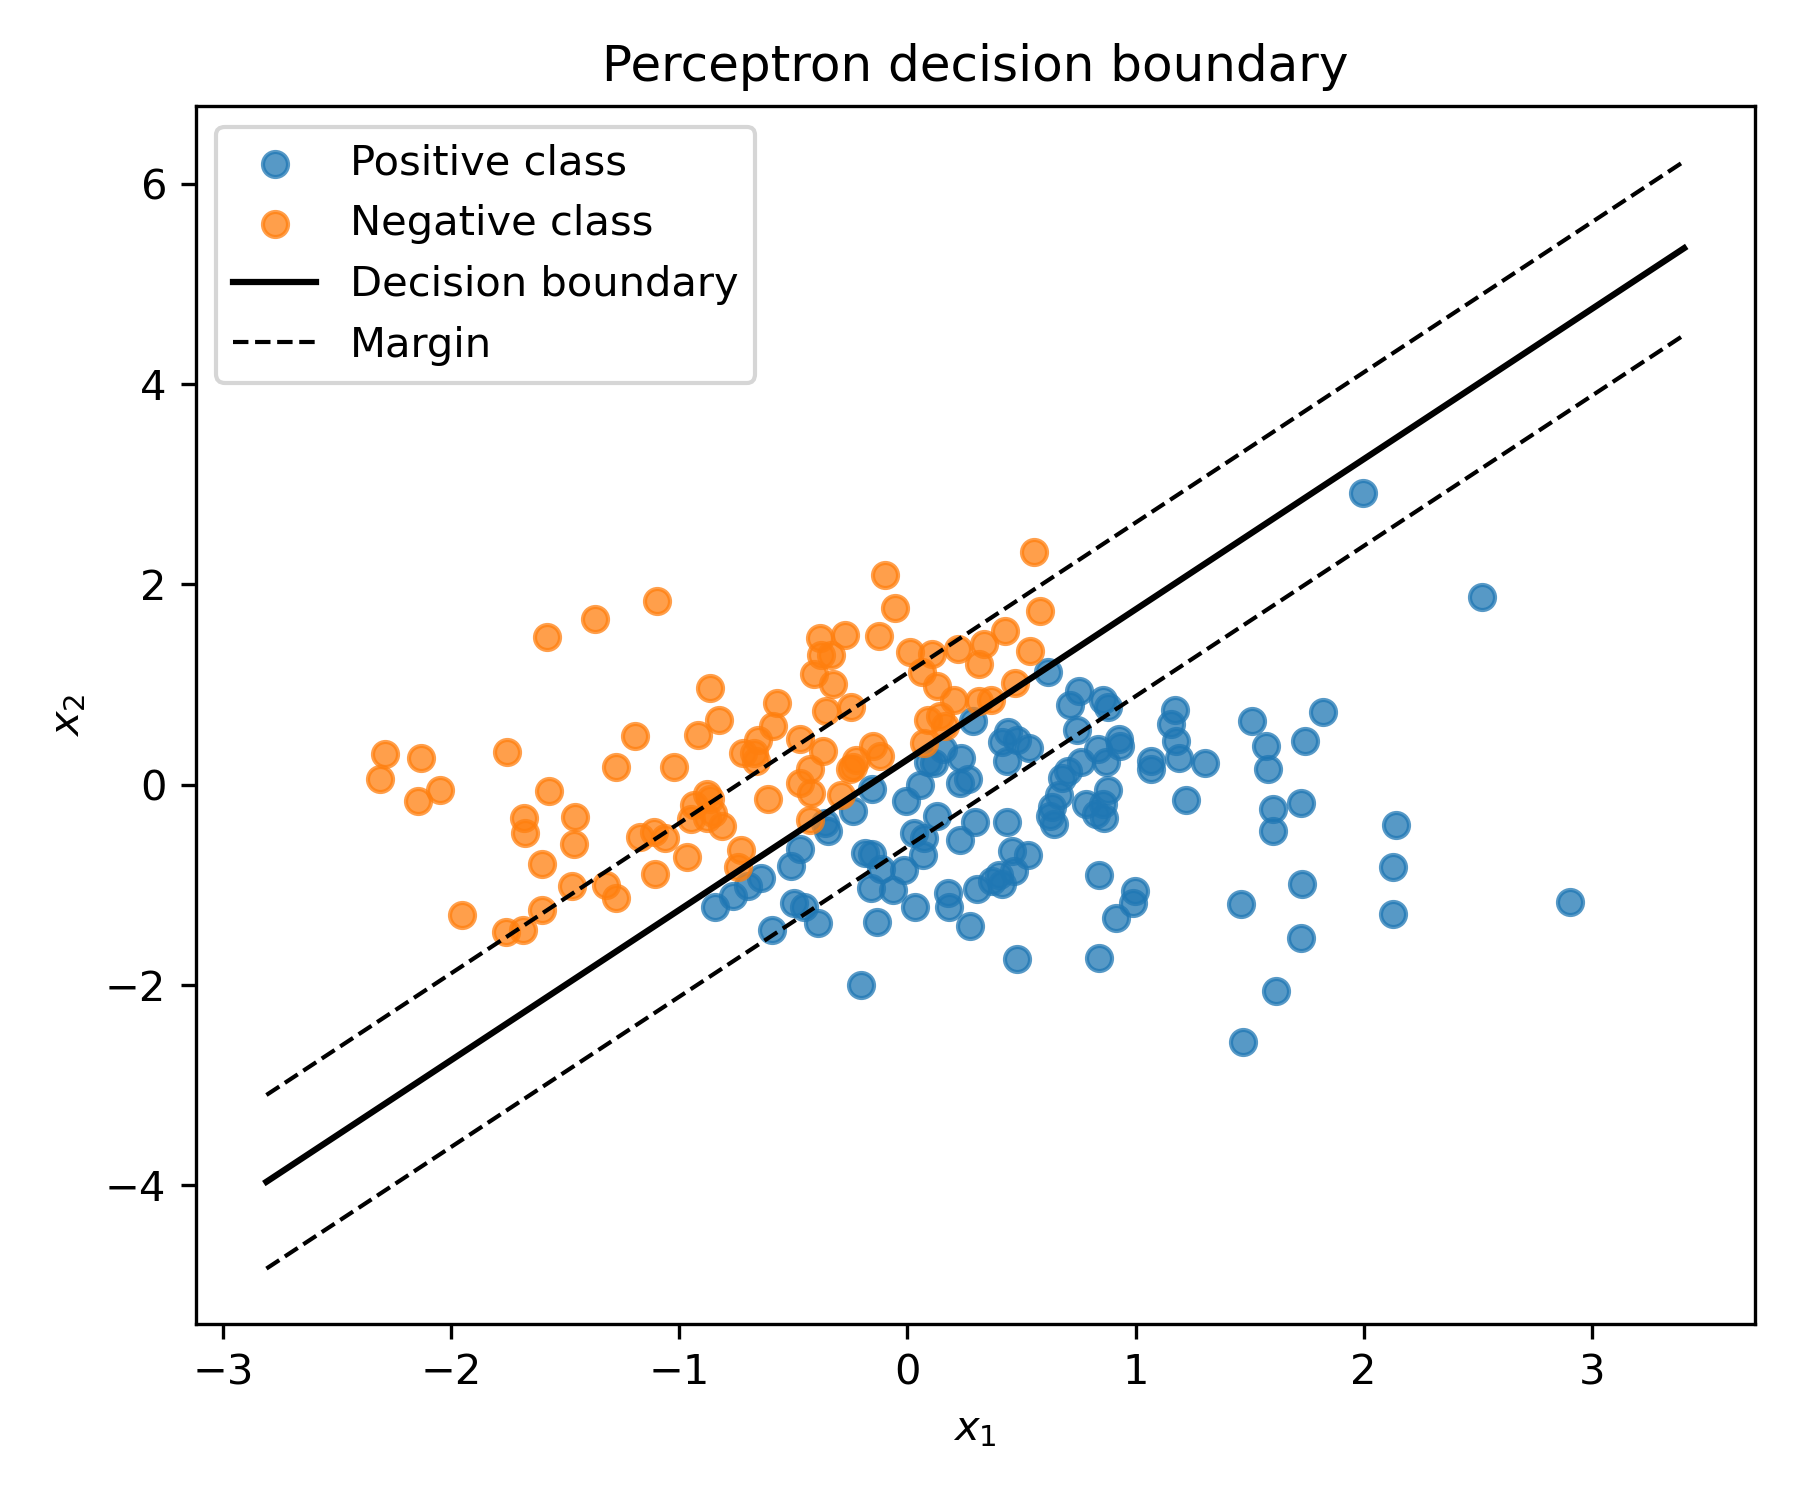
\includegraphics[width=0.7\textwidth]{perceptron_decision_boundary.png}
  \caption{Perceptron decision boundary separating two classes with margin intuition.}
  \label{fig:perceptron_decision_boundary}
\end{figure}
\FloatBarrier

\section{Multilayer Perceptron (MLP) and Forward Propagation}
An MLP stacks layers of perceptrons with differentiable activation functions, enabling the model to approximate complex nonlinear mappings. Given an $L$-layer MLP, the computation proceeds layer by layer:
\begin{align}
  \mathbf{a}^{(1)} &= \mathbf{W}^{(1)}\mathbf{x} + \mathbf{b}^{(1)}, & \mathbf{h}^{(1)} &= \phi^{(1)}\bigl(\mathbf{a}^{(1)}\bigr), \\
  \mathbf{a}^{(\ell)} &= \mathbf{W}^{(\ell)}\mathbf{h}^{(\ell-1)} + \mathbf{b}^{(\ell)}, & \mathbf{h}^{(\ell)} &= \phi^{(\ell)}\bigl(\mathbf{a}^{(\ell)}\bigr), \\
  \hat{\mathbf{y}} &= \mathbf{h}^{(L)},
\end{align}
where $\phi^{(\ell)}$ denotes the element-wise activation of layer $\ell$.

\subsection{Forward Propagation Algorithm}
Forward propagation evaluates the network efficiently by reusing intermediate results.

\begin{lstlisting}[language=Python, caption={Forward pass for a dense MLP.}]
import numpy as np

def forward_pass(weights, biases, activations, x):
    h = x
    for W, b, act in zip(weights, biases, activations):
        a = W @ h + b
        h = act(a)
    return h
\end{lstlisting}

\subsection{Expressive Power}
The universal approximation theorem states that a feedforward network with a single hidden layer containing a finite number of neurons can approximate any continuous function on compact subsets of $\mathbb{R}^n$ given appropriate activation functions. Deeper networks reduce the number of neurons required by reusing intermediate abstractions.

\begin{figure}[H]
  \centering
  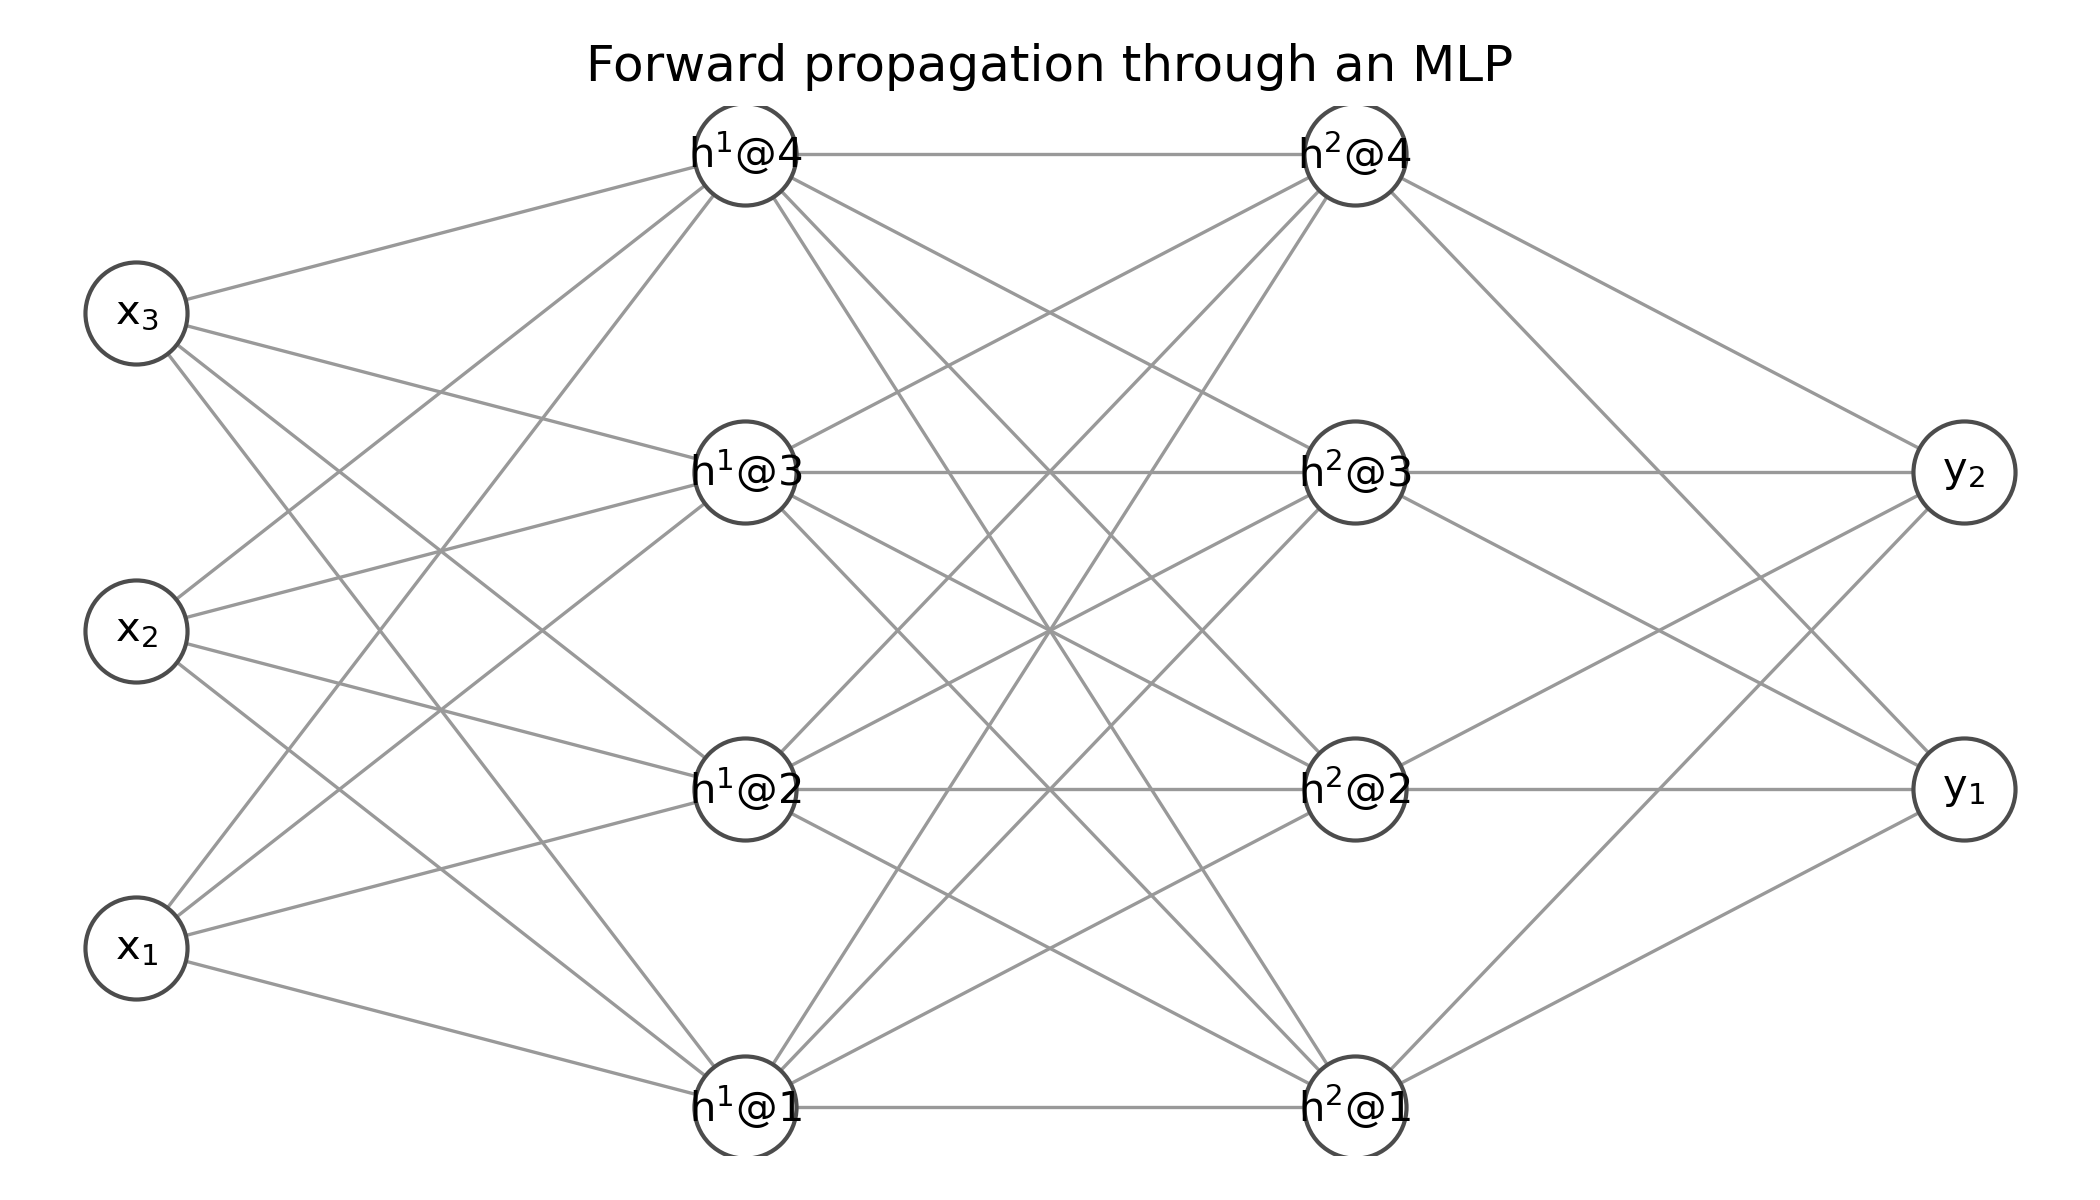
\includegraphics[width=0.8\textwidth]{mlp_forward_pass.png}
  \caption{Forward propagation through an MLP with highlighted linear maps and activations.}
  \label{fig:mlp_forward_pass}
\end{figure}
\FloatBarrier

\section{Activation Functions}
Activation functions inject nonlinearity, enabling neural networks to model complex relationships. Figure~\ref{fig:activation_functions} compares several common activations.

\subsection{Sigmoid}
The logistic sigmoid maps real numbers to $(0,1)$:
\begin{equation}
  \sigma(z) = \frac{1}{1 + e^{-z}}, \quad \sigma'(z) = \sigma(z)\bigl(1-\sigma(z)\bigr).
\end{equation}
It saturates for large $|z|$, which can slow training.

\subsection{Hyperbolic Tangent}
The tanh activation rescales the sigmoid to $(-1,1)$ and is zero-centered:
\begin{equation}
  \tanh(z) = \frac{e^{z} - e^{-z}}{e^{z} + e^{-z}}, \quad \frac{d}{dz}\tanh(z) = 1 - \tanh^2(z).
\end{equation}

\subsection{Rectified Linear Unit (ReLU)}
ReLU is defined as
\begin{equation}
  \mathrm{ReLU}(z) = \max(0, z), \quad \mathrm{ReLU}'(z) = \begin{cases}1,& z>0,\\0,& z<0.\end{cases}
\end{equation}
It accelerates convergence but suffers from ``dead'' neurons when $z<0$ persistently.

\subsection{Leaky ReLU}
Leaky ReLU mitigates dead neurons by allowing a small slope for negative inputs:
\begin{equation}
  \mathrm{LeakyReLU}(z) = \begin{cases} z,& z \ge 0,\\ \alpha z,& z < 0,\end{cases}
\end{equation}
with $\alpha \approx 0.01$.

\subsection{Gaussian Error Linear Unit (GELU)}
GELU weights inputs by their magnitude and probability under a standard Gaussian:
\begin{equation}
  \mathrm{GELU}(z) = z \Phi(z) = \frac{z}{2}\left[1 + \mathrm{erf}\left(\frac{z}{\sqrt{2}}\right)\right],
\end{equation}
where $\Phi$ is the Gaussian cumulative distribution function and $\mathrm{erf}$ is the error function. GELU maintains smooth derivatives, facilitating optimization in transformer architectures.

\begin{figure}[H]
  \centering
  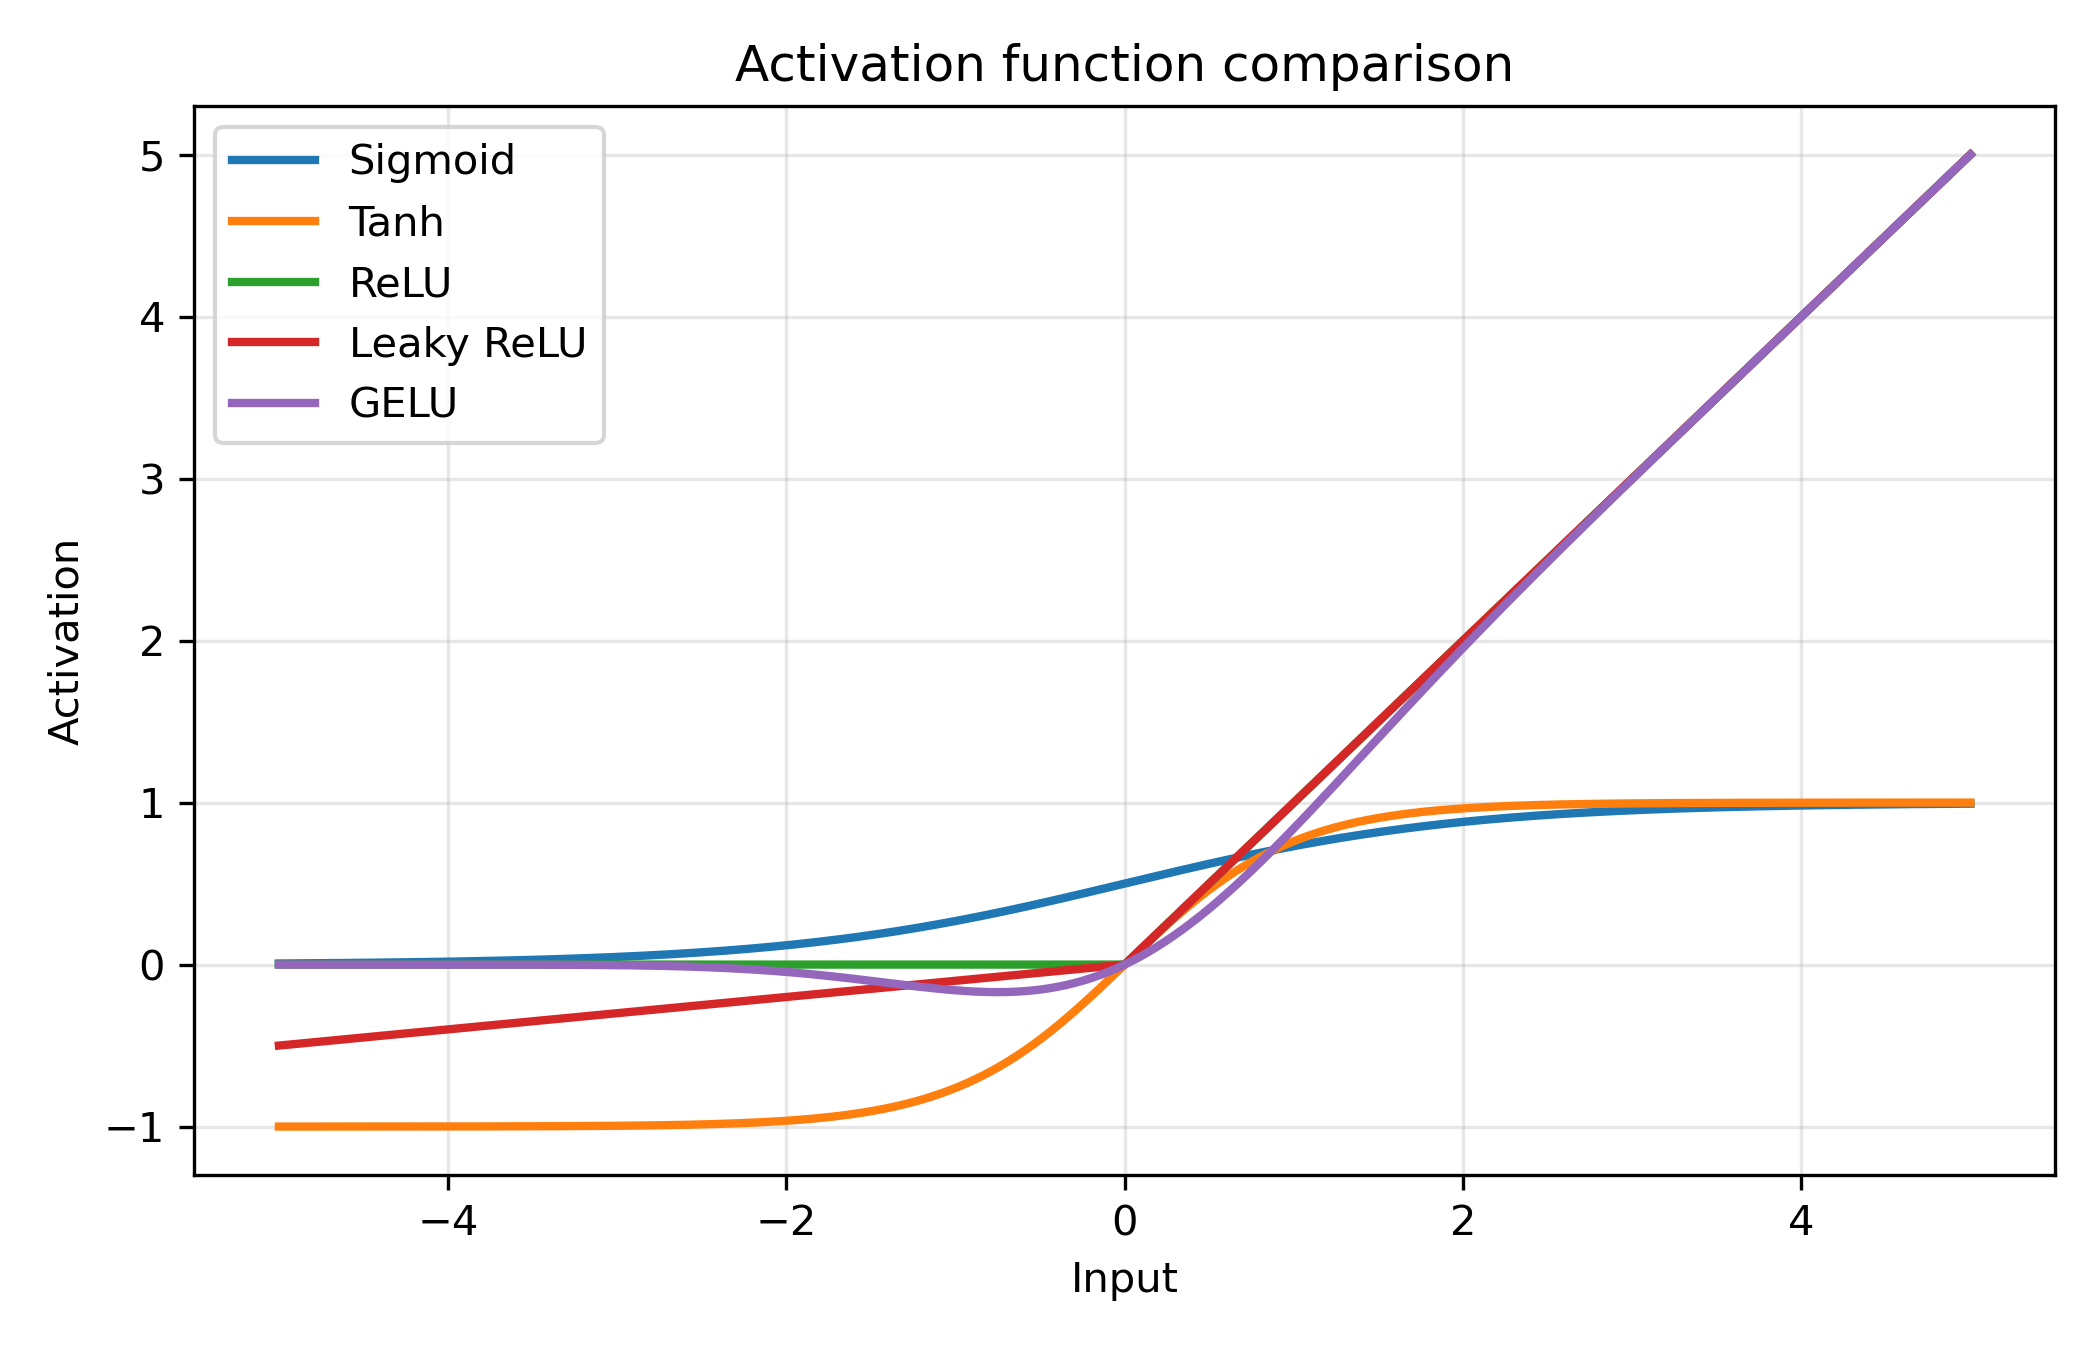
\includegraphics[width=0.8\textwidth]{activation_functions.png}
  \caption{Comparison of common activation functions.}
  \label{fig:activation_functions}
\end{figure}
\FloatBarrier

\section{Loss Functions}
Loss functions quantify the discrepancy between predictions and targets, guiding gradient-based optimization.

\subsection{Mean Squared Error (MSE)}
For regression with targets $t_i$ and predictions $\hat{y}_i$, the MSE is
\begin{equation}
  \mathcal{L}_{\mathrm{MSE}} = \frac{1}{N} \sum_{i=1}^{N} \bigl(\hat{y}_i - t_i\bigr)^2.
\end{equation}
The gradient with respect to $\hat{y}_i$ is $\frac{2}{N}(\hat{y}_i - t_i)$.

\subsection{Cross-Entropy Loss}
For binary classification with targets $t_i \in \{0,1\}$ and predicted probabilities $p_i$, the binary cross-entropy loss reads
\begin{equation}
  \mathcal{L}_{\mathrm{BCE}} = -\frac{1}{N} \sum_{i=1}^{N} \left[t_i \log p_i + (1-t_i) \log(1-p_i)\right].
\end{equation}
When combined with the logistic sigmoid, this loss aligns the gradient with the negative log-likelihood of a Bernoulli distribution.

For multi-class classification with softmax outputs $p_{i,k}$ over classes $k$, the categorical cross-entropy is
\begin{equation}
  \mathcal{L}_{\mathrm{CE}} = -\frac{1}{N} \sum_{i=1}^{N} \sum_{k=1}^{K} t_{i,k} \log p_{i,k},
\end{equation}
where $t_{i,k}$ is the one-hot target.

\subsection{Huber Loss}
The Huber loss interpolates between L1 and L2 losses, offering robustness to outliers while retaining differentiability at the origin:
\begin{equation}
  \mathcal{L}_{\delta}(r) = \begin{cases}
    \tfrac{1}{2} r^2, & |r| \le \delta, \\
    \delta(|r| - \tfrac{1}{2}\delta), & |r| > \delta,
  \end{cases}
\end{equation}
where $r = \hat{y} - t$ and $\delta$ controls the transition point.

\begin{figure}[H]
  \centering
  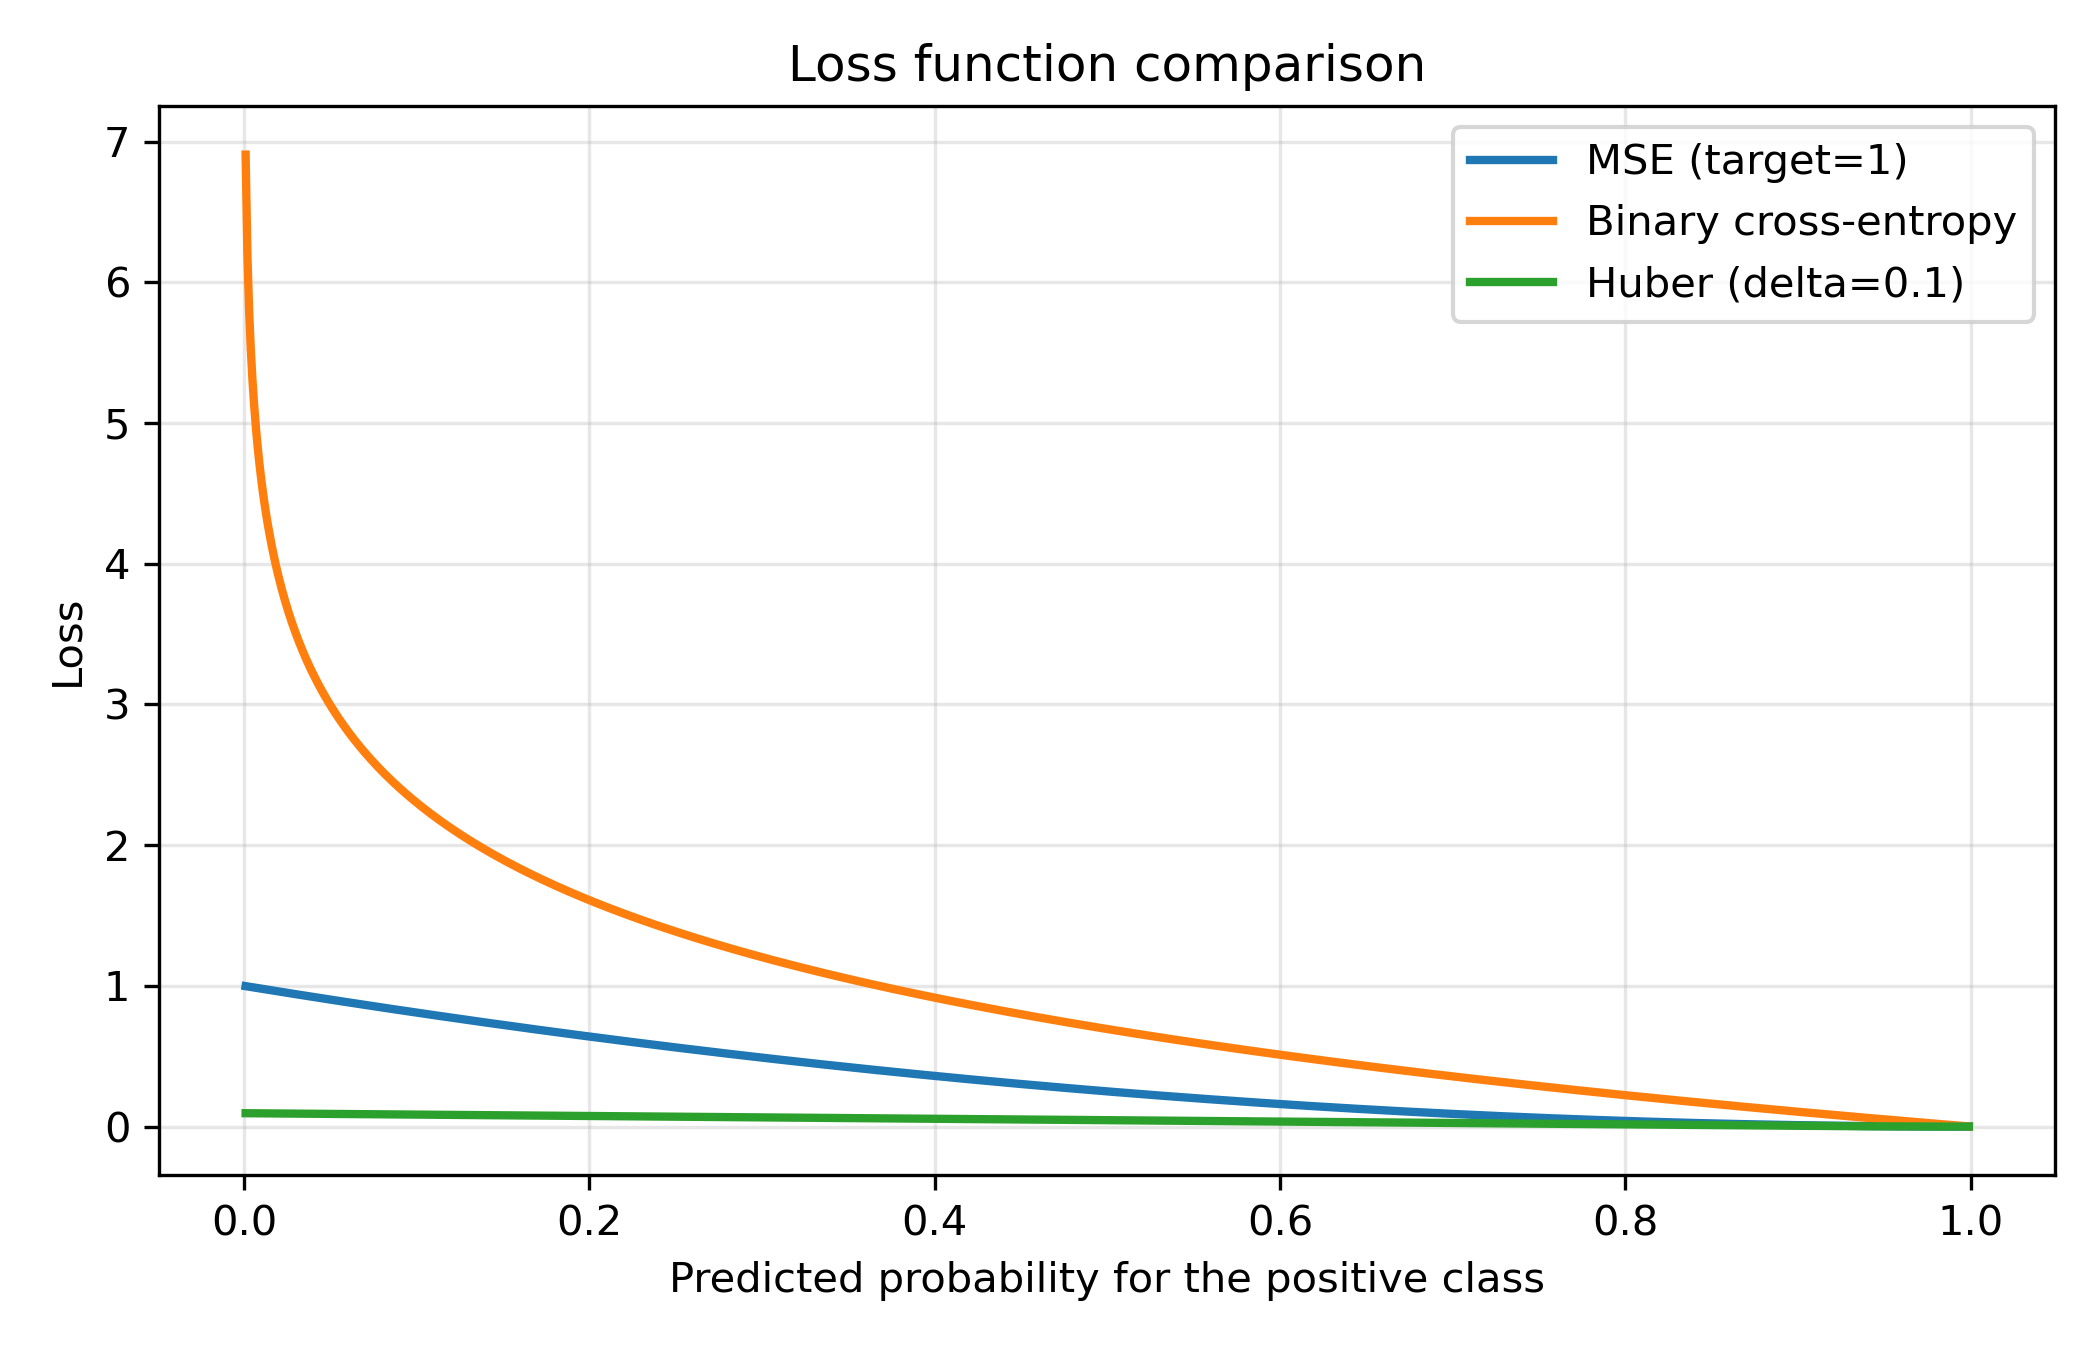
\includegraphics[width=0.8\textwidth]{loss_functions.png}
  \caption{Shapes of MSE, cross-entropy (binary log-loss), and Huber losses.}
  \label{fig:loss_functions}
\end{figure}
\FloatBarrier

\section{Practical Considerations}
\begin{itemize}
  \item \textbf{Initialization:} Proper weight initialization (e.g., Xavier or He) prevents activations from vanishing or exploding.
  \item \textbf{Normalization:} Batch or layer normalization stabilizes training by controlling activation statistics.
  \item \textbf{Optimization:} Adaptive optimizers (Adam, RMSprop) adjust learning rates per parameter.
  \item \textbf{Regularization:} Techniques such as dropout, weight decay, or early stopping combat overfitting.
\end{itemize}

\end{document}
